
%*************************************************************************
%
%   SEE CALIBRATION_1 FOR THE FIRST PART (COMMENTED HEREAFTER)
%
%************************************************************************


%----------------------------------------------------------------------------------------
%	8./ Calibration
%----------------------------------------------------------------------------------------
%\section{Calibration}
%\label{se:calibration}

%We present the calibration of the absolute scale of the flux densities
%for the NIKA2 instrument in this section using Uranus as the main
%primary calibrator. Practically, at the stage of the FOV
%reconstruction (see Sect.~\ref{se:geometry}), an absolute
%coefficient factor per detectors is derived using a \bm\ scan of
%Uranus. This step realizes also the inter-calibration of all the KID,
%as the coefficient factors give the KID gains. Secondly, the flux
%density absolute scale is further refined by monitoring the primary
%calibrator all along the observation campaign to estimate an
%absolute calibration correction.

%We have evidenced a daily variation of the absolute calibration
%coefficients as a function of the observation date, which is related
%to temperature-induced variation of the beam size. If left uncorrected, this variation
%induces a sizable increase of the calibration uncertainties. To
%overcome this issue, we primarily flag the most impacted observation
%dates and exclude the observations acquired during these periods. This
%conservative approach constitutes the baseline calibration method,
%which is further used for the performance assessment. For cross-check,
%we also proposed an alternative method relying on a photometric
%correction depending on the beam size. Both approaches require an
%accurate monitoring of the beam size as a function of the observation
%date.


%First we describe the method for the absolute calibration in
%Sect.~\ref{se:calibration_method}, then we present the
%inter-calibration and the flat fields in
%Sect.~\ref{se:flat_field}. The temperature-induced variation and the
%beam size monitoring are then discussed in
%Sect.~\ref{se:beam_variation}. Finally, the baseline calibration is
%presented in Sect.~\ref{se:baseline_calibration} and the calibration
%with a photometric correction in
%Sect.~\ref{se:photometric_correction}.  



%---------------------------------------------------------------------
%	Method
%---------------------------------------------------------------------

%\subsection{Absolute calibration procedure and photometric system}
%\label{se:calibration_method}

%\subsubsection{Photometric system}
%\label{se:photometric_system}

%\subsubsection{Color correction}
%

%\subsubsection{Diffuse source}
%\label{se:extended_source_calib}

%\subsubsection{Practical calibration}
%

%---------------------------------------------------------------------
%	INTERCALIBRATION
%---------------------------------------------------------------------
%\subsection{Relative calibration \& flat fields}
%\label{se:flat_field}


%---------------------------------------------------------------------
%	TEMPERATURE-INDUCED VARIATION
%---------------------------------------------------------------------
%\subsection{Temperature-induced variations}
%\label{se:beam_variation}

%\subsubsection{Beam monitoring using bright source scans}
%\label{se:beam_monitoring_otf}

%\subsubsection{Beam monitoring using pointing}
%\label{se:beam_monitoring_pointing}


%---------------------------------------------------------------------
%	BASELINE CALIBRATION
%---------------------------------------------------------------------
\subsection{Baseline calibration}
\label{se:baseline_calibration}

To assess NIKA2 performance, we rely on a baseline calibration that
resorts to the following methods: i) the calibration in FWHM$_0$ Gaussian
as detailed in Sect.~\ref{se:calibration_method} is implemented, ii)
the temperature-induced variation effect is mitigated using the scan
selection described in Sect.~\ref{se:data_selection} and iii) the
atmospheric attenuation is corrected using the {\tt corrected skydip}
opacity derivation described in Sect.~\ref{se:corrected-skydip}.

In this section, we check the stability of Uranus flux density
estimates againts the beam size in
Sect.~\ref{se:baseline_calibration_scans} and againts the
atmospheric transmission in
Sect.~\ref{se:baseline_calibration_atm}. In
Sect.~\ref{se:baseline_calibration_opacity}, we compare
Uranus flux density estimates after absolute calibration using other
opacity correction methods.

\subsubsection{Flux stability against the beam size}
\label{se:baseline_calibration_scans}
We present Uranus measured-to-predicted flux density ratios as a
function of the 2D Gaussian FWHM estimates and color-coded from the
observation dates given in UT hours in
Fig.~\ref{fig:calib_uranus_vs_fwhm_all}.

\begin{figure}[!htbp]
\begin{center}
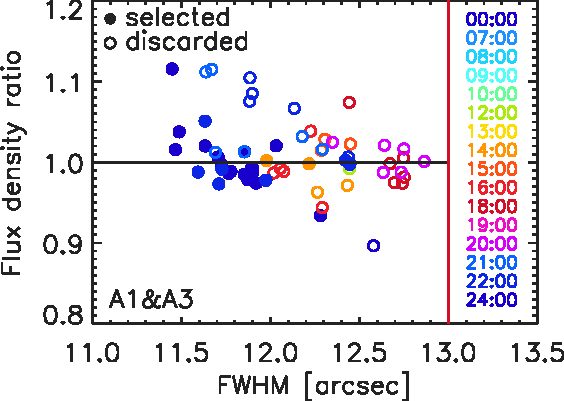
\includegraphics[clip=true, trim={0, -0.3cm, -0.3cm, 0}, width=0.525\linewidth]{Figures/plot_flux_density_ratio_fwhm_uranus_corrected_skydip_narrow_1mm.pdf}
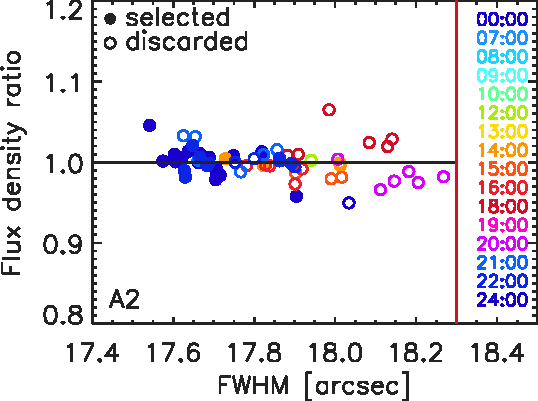
\includegraphics[clip=true, trim={0.7cm, -0.3cm, -0.25cm, 0}, width=0.465\linewidth]{Figures/plot_flux_density_ratio_fwhm_uranus_corrected_skydip_narrow_a2.pdf}
\caption[Uranus flux density stability against FWHM]{ Uranus flux
density ratio vs beam size after the baseline calibration. The ratio
of Uranus measured flux densities to expectations in function of the
measured 2D Gaussian beam FWHM is shown for the $1$-mm array
combination and for array 2 after absolute calibration using the
baseline method. These plots include all Uranus scans acquired during
N2R9, N2R12 and N2R14 campaigns and whose beam FWHM are below the threshold indicated
by the vertical red lines (open circles), as well as the scans that
met the baseline selection criteria (filled circles).}
\label{fig:calib_uranus_vs_fwhm_all}
\end{center}
\end{figure}

The flux density estimates have been calibrated beforehands, so that
the flux density ratios are equal to unity in average by construction.
The selected scan flux ratios (shown as full circles) are stable
against the beam FWHM. The baseline scan selection of
Sect.~\ref{se:data_selection} is thus efficient to mitigate the
temperature-induced beam variation effect.


\subsubsection{Flux stability against the atmospheric transmission}
\label{se:baseline_calibration_atm}

We test the stability of Uranus flux densities calibrated using the
baseline calibration against the atmospheric transmission. The later
quantity, we
recall, depends on the measured zenith opacity $\tau$ and the scan
average airmass $x = $cosec$(\delta)$ as $\exp{(-\tau \cdot x)}$. In
the first row of Fig.~\ref{fig:calib_uranus_vs_atmtrans}, Uranus flux ratios
are plotted as a function of the atmospheric
transmission for the $1$-mm array combination and Array 2 and for the
three considered observation campaigns (N2R9, N2R12 $\&$ N2R14). No
sizable dependencies of the flux ratio on the atmospheric transmission
is observed, which constitutes a first
indication of the robustness of the flux density estimates against the
atmospheric conditions using the baseline calibration. This will be
further tested using more scans in Sect.~\ref{se:photometry}.
%
\begin{figure}[!htbp]
\begin{center}
  % corrected skydip
  \begin{overpic}[clip=true, trim={0, -0.3cm, -0.3cm, 0}, width=0.49\linewidth]{Figures/plot_flux_density_ratio_obstau_uranus_corrected_skydip_narrow_1mm.pdf}
    \put(20,23){\footnotesize Baseline}
  \end{overpic}
  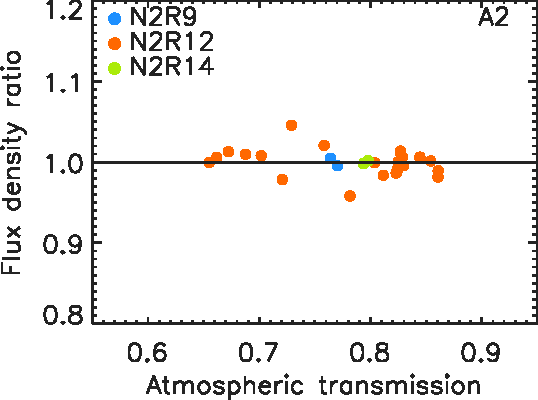
\includegraphics[clip=true, trim={0, -0.3cm, -0.3cm, 0}, width=0.49\linewidth]{Figures/plot_flux_density_ratio_obstau_uranus_corrected_skydip_narrow_a2.pdf}
  % taumeter
  \begin{overpic}[clip=true, trim={0, -0.3cm, -0.3cm, 0}, width=0.49\linewidth]{Figures/plot_flux_density_ratio_obstau_uranus_tau225_narrow_1mm.pdf}
    \put(20,23){\footnotesize Taumeter}
  \end{overpic}
  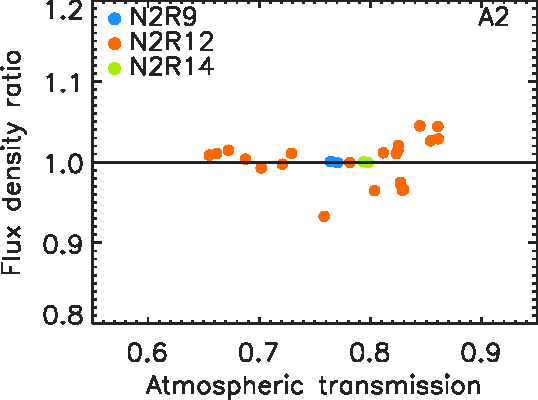
\includegraphics[clip=true, trim={0, -0.3cm, -0.3cm, 0}, width=0.49\linewidth]{Figures/plot_flux_density_ratio_obstau_uranus_tau225_narrow_a2.pdf}
  % skydip
  \begin{overpic}[clip=true, trim={0, -0.3cm, -0.3cm, 0}, width=0.49\linewidth]{Figures/plot_flux_density_ratio_obstau_uranus_skydip_narrow_1mm.pdf}
    \put(20,23){\footnotesize Skydip}
  \end{overpic}
  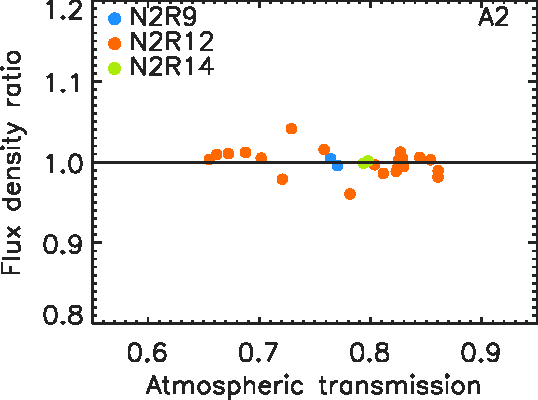
\includegraphics[clip=true, trim={0, -0.3cm, -0.3cm, 0}, width=0.49\linewidth]{Figures/plot_flux_density_ratio_obstau_uranus_skydip_narrow_a2.pdf}
  \caption[Uranus flux density stability against atmospheric
    transmission]{Uranus flux density ratio vs atmospheric transmission
    shown for the $1$-mm array
    combination (left column) and for array 2 (right column) after absolute
    calibration using (\emph{first row}:) the baseline method, (\emph{second row}:) the 'taumeter'-based and
    (\emph{third row}:) the 'skydip'-based methods. These plots
    include all Uranus scans acquired during N2R9, N2R12 and N2R14
    campaigns. }
  \label{fig:calib_uranus_vs_atmtrans}
\end{center}
\end{figure}
%


\subsubsection{Comparison with other opacity correction methods}
\label{se:baseline_calibration_opacity}

For cross-check, we have derived the absolute
calibration factors using the {\tt taumeter}
(Sect.~\ref{se:taumeter-method}) and the {\tt skydip}
(Sect.~\ref{se:skydip-method}) opacity
correction methods. We then compare Uranus
flux density estimates after absolute calibration using the baseline
calibration and these two alternative
calibrations. Figure~\ref{fig:calib_uranus_vs_atmtrans}
shows Uranus measured-to-modeled
flux ratio as a function of the atmospheric transmission for A1$\&$A3
and for A2 after the {\tt taumeter}-based calibration (second row) and
after the {\tt skydip}-based calibration (third row). We observe more
dispersion for the {\tt taumeter}-based flux ratio, whereas the {\tt
skydip}-based ratios are very similar as the baseline ratios except
for a slight decrease of the flux at low atmospheric
transmission. Thus the {\tt taumeter} and {\tt skydip} methods can be used for
the absolute calibration in complement to the baseline method, e.g. to
perform robustness tests as in Sect.~\ref{se:photometry}. 



%---------------------------------------------------------------------
%	PHOTOMETRIC CORRECTION
%---------------------------------------------------------------------
\subsection{Photometric correction}
\label{se:photometric_correction}
